% !TEX root = ../FundationsDataScience.tex

\chapter{Inverse Problems}

The main references for this chapter are~\cite{mallat2008wavelet,scherzer2009variational,engl1996regularization}.

%%%%%%%%%%%%%%%%%%%%%%%%%%%%%%%%%%%%%%%%%%%%%%%%%%%%%%%%%%%%%%%%
%%%%%%%%%%%%%%%%%%%%%%%%%%%%%%%%%%%%%%%%%%%%%%%%%%%%%%%%%%%%%%%%
%%%%%%%%%%%%%%%%%%%%%%%%%%%%%%%%%%%%%%%%%%%%%%%%%%%%%%%%%%%%%%%%
\section{Inverse Problems Regularization}

Increasing the resolution of signals and images requires to solve an ill posed inverse problem. This corresponds to inverting a linear measurement operator that reduces the resolution of the image. This chapter makes use of convex regularization introduced in Chapter \ref{chap-variational} to stabilize this inverse problem.

We consider a (usually) continuous linear map $\Phi : \Ss \rightarrow \Hh$ where $\Ss$ can be an Hilbert or a more general Banach space.
%
This operator is intended to capture the hardware acquisition process, which maps a high resolution unknown signal $f_0 \in \Ss$ to a noisy low-resolution obervation 
\eq{
	y = \Phi f_0 + w \in \Hh
}
where $w \in \Hh$ models the acquisition noise. In this section, we do not use a random noise model, and simply assume that $\norm{w}_\Hh$ is bounded.

In most applications, $\Hh=\RR^P$ is finite dimensional, because the hardware involved in the acquisition can only record a finite (and often small) number $P$ of observations.
%
Furthermore, in order to implement numerically a recovery process on a computer, it also makes sense to restrict the attention to $\Ss=\RR^N$,  where $N$ is number of point on the discretization grid, and is usually very large, $N \gg P$. 
%
However, in order to perform a mathematical analysis of the recovery process, and to be able to introduce meaningful models on the unknown $f_0$, it still makes sense to consider infinite dimensional functional space (especially for the data space $\Ss$).

The difficulty of this problem is that the direct inversion of $\Phi$ is in general impossible or not advisable because $\Phi^{-1}$ have a large norm or is even discontinuous. This is further increased by the addition of some measurement noise $w$, so that the relation $\Phi^{-1} y=f_0+\Phi^{-1}w$ would leads to an explosion of the noise $\Phi^{-1}w$.

We now gives a few representative examples of forward operators $\Phi$.

%%%
\paragraph{Denoising.}

The case of the identity operator $\Phi=\Id_\Ss$, $\Ss=\Hh$ corresponds to the classical denoising problem, already treated in Chapters \ref{chap-denoising}�and \ref{chap-variational}. 

%%%
\paragraph{De-blurring and super-resolution.}

For a general operator $\Phi$, the recovery of $f_0$ is more challenging, and this requires to perform both an inversion and a denoising. For many problem, this two goals are in contradiction, since usually inverting the operator increases the noise level.
%
This is for instance the case for the deblurring problem, where $\Phi$ is a translation invariant operator, that corresponds to a low pass filtering with some kernel $h$
\eql{\label{eq-deblurring-operator}
	\Phi f = f \star h.
}
One can for instance consider this convolution over $\Ss=\Hh=L^2(\TT^d)$, see Proposition~\ref{prop-ti-convol-l2}. 
%
In practice, this convolution is followed by a sampling on a grid $\Phi f = \enscond{(f \star h)(x_k)}{0 \leq k< P}$, see Figure \ref{fig-ip}, middle, for an example of a low resolution image $\Phi f_0$.
%
Inverting such operator has important industrial application to upsample the content of digital photos and to compute high definition videos from low definition videos.


%%%
\paragraph{Interpolation and inpainting.}

Inpainting corresponds to interpolating missing pixels in an image. This is modelled by a diagonal operator over the spacial domain
\eql{\label{eq-inp-operator}
	(\Phi f)(x) = \choice{
	0 \qifq x \in \Om,\\
	f(x) \qifq x \notin \Om.
	}
}
where $\Om \subset [0,1]^d$ (continuous model) or $\{0,\ldots,N-1\}$ which is then a set of missing pixels.
%
Figure \ref{fig-ip}, right, shows an example of damaged image $\Phi f_0$.

\myfigure{
\tabtrois{
\image{invpbm}{.3}{ip-sample-image}&
\image{invpbm}{.3}{ip-sample-superresol}&
\image{invpbm}{.3}{ip-sample-inpainting}\\
Original $f_0$ & Low resolution $\Phi f_0$ & Masked $\Phi f_0$
}
}{%
	Example of inverse problem operators. %	
}{fig-ip}


%%%
\paragraph{Medical imaging.}

Most medical imaging acquisition device only gives indirect access to the signal of interest, and is usually well approximated by such a linear operator $\Phi$.
%
In scanners, the acquisition operator is the Radon transform, which, thanks to the Fourier slice theorem, is equivalent to partial Fourier mesurments along radial lines.
% 
Medical resonance imaging (MRI) is also equivalent to partial Fourier measures
\eql{\label{eq-inp-operator}
	\Phi f= \enscond{ \hat f(x) }{ x \in \Om }.
}
Here, $\Om$ is a set of radial line for a scanner, and smooth curves (e.g. spirals) for MRI. 

Other indirect application are obtained by electric or magnetic fields measurements of the brain activity (corresponding to MEG/EEG). Denoting $\Om \subset \RR^3$ the region around which measurements are performed (e.g. the head), in a crude approximation of these measurements, one can assume $\Phi f = \enscond{(\psi \star f)(x)}{x \in \partial \Om}$ where $\psi(x)$ is a kernel accounting for the decay of the electric or magnetic field, e.g. $\psi(x)=1/\norm{x}^2$. 

%%%%%%%%%%%%%%%%%%%%%%%%%%%%%%%%%%%%%%%%%%%%%%%%%%%%%%%%%%%%%%%%
%%%%%%%%%%%%%%%%%%%%%%%%%%%%%%%%%%%%%%%%%%%%%%%%%%%%%%%%%%%%%%%%
%%%%%%%%%%%%%%%%%%%%%%%%%%%%%%%%%%%%%%%%%%%%%%%%%%%%%%%%%%%%%%%%
\section{Theoretical Study of Quadratic Regularization}

We now give a glimpse on the typical approach to obtain theoretical guarantee on recovery quality in the case of Hilbert space. The goal is not to be exhaustive, but rather to insist on the modelling hypotethese, namely smoothness implies a so called ``source condition'', and the inherent limitations of quadratic methods (namely slow rates and the impossibility to recover information in $\ker(\Phi)$, i.e. to achieve super-resolution). 

%%%%%%%%%%%%%%%%%%%%%%%%%%%%%%%%%%%%%%%%%%%%%%%%%%%%%%%%%%%%%%%%
\subsection{Singular Value Decomposition}


%%%%%%%%%%
\paragraph{Finite dimension.}

Let us start by the simple finite dimensional case $\Phi \in \RR^{P \times N}$ so that $\Ss=\RR^N$ and $\Hh=\RR^P$ are Hilbert spaces.
%
In this case, the Singular Value Decomposition (SVD) is the key to analyze the operator very precisely, and to describe linear inversion process.  

\begin{prop}[SVD]
	There exists $(U,V) \in \RR^{N \times R} \times \RR^{P \times R}$, where $R=\rank(\Phi)=\dim(\Im(\Phi))$, with $U^\top U=V^\top V=\Id_R$, i.e. having orthogonal columns $(u_m)_{m=1}^R \subset \RR^N, (v_m)_{m=1}^R \subset \RR^P$,  and $(\si_m)_{m=1}^R$ with $\si_m>0$, such that
	\eql{\label{eq-svd-expan}
		\Phi = U\diag_m(\si_m) V^\top = \sum_{m=1}^R \si_m u_m v_m^\top.
	}
\end{prop}

\begin{proof}
	We first analyze the problem, and notice that if $\Phi = U \Si V^\top$ with $\Si = \diag_m(\si_m)$, then 
	$\Phi\Phi^\top=U \Si^2 U^\top$ and then $V^\top = \Si^{-1} U^\top \Phi$.
	%
	We can use this insight. Since $\Phi\Phi^\top$ is a positive symmetric matrix, we write its eigendecomposition as $\Phi\Phi^\top=U \Si^2 U^\top$ where $\Si = \diag_{m=1}^R(\si_m)$ with $\si_m>0$. We then define $V \eqdef \Phi^\top U \Si^{-1}$.
	% 
	One then verifies that 
	\eq{
		V^\top V = (\Si^{-1} U^\top \Phi)  (\Phi^\top U \Si^{-1}) = 
			\Si^{-1} U^\top (U \Si^2 U^\top) U \Si^{-1} = \Id_P
		\qandq
		U \Si V^\top = U \Si \Si^{-1} U^\top \Phi  = \Phi.
	} 
\end{proof}

This theorem is still valid with complex matrice, replacing $^\top$ by $^*$.
%
Expression~\eqref{eq-svd-expan} describes $\Phi$ as a sum of rank-1 matrices $u_m v_m^\top$.
%
One usually order the singular values $(\si_m)_m$ in decaying order $\si_1 \geq \ldots \geq \si_R$. If these values are different, then the SVD is unique up to $\pm 1$ sign change on the singular vectors.  

The left singular vectors $U$ is an orthonormal basis of $\Im(\Phi)$, while the right singular values is an orthonormal basis of $\Im(\Phi^\top)=\ker(\Phi)^\bot$.
%
The decomposition~\eqref{eq-svd-expan} is often call the ``reduced'' SVD because one has only kept the $R$ non-zero singular values.
The ``full'' SVD is obtained by completing $U$ and $V$ to define orthonormal bases of the full spaces $\RR^P$ and $\RR^N$. Then $\Si$ becomes a rectangular matrix of size $P\times N$.

A typical example is for $\Phi f=f \star h$ over $\RR^P=\RR^N$, in which case the Fourier transform diagonalizes the convolution, i.e.
\eql{\label{eq-diag-filter-finite}
	\Phi = (u_m)_m^* \diag(\hat h_m) (u_m)_m
}
where $(u_m)_n \eqdef \frac{1}{\sqrt{N}}e^{\frac{2\imath\pi}{N}nm}$ so that the singular values are $\si_m=|\hat h_m|$ (removing the zero values) and the singular vectors are $(u_m)_n$ and $(v_m \th_m)_n$ where $\th_m \eqdef |\hat h_m|/\hat h_m$ is a unit complex number. 

Computing the SVD of a full matrix $\Phi \in \RR^{N \times N}$ has complexity $N^3$. 

%%%%%%%%%%
\paragraph{Compact operators.}

One can extend the decomposition to compact operators $\Phi : \Ss \rightarrow \Hh$ between separable Hilbert space. A compact operator is such that $\Phi B_1$ is pre-compact where $B_1=\enscond{s \in \Ss}{\norm{s}\leq 1}$ is the unit-ball. This means that for any sequence $(\Phi s_k)_k$ where $s_k \in B_1$ one can extract a converging sub-sequence. Note that in infinite dimension, the identity operator $\Phi : \Ss \rightarrow \Ss$ is never compact.

Compact operators $\Phi$ can be shown to be equivalently defined as those for which an expansion of the form~\eqref{eq-svd-expan} holds
\eql{\label{eq-svd-operators}
 	\Phi = \sum_{m=1}^{+\infty} \si_m u_m v_m^\top
}
where $(\si_m)_m$ is a decaying sequence onverging to $0$, $\si_m \rightarrow 0$.
%
Here in~\eqref{eq-svd-operators} convergence holds in the operator norm, which is the algebra norm on linear operator inherited from those of $\Ss$ and $\Hh$
\eq{
	\norm{\Phi}_{\Ll(\Ss,\Hh)} \eqdef \umin{ \norm{\Phi u}_\Hh }{ \norm{u}_\Ss \leq 1 }.
}
For $\Phi$ having an SVD decomposition~\eqref{eq-svd-operators}, $\norm{\Phi}_{\Ll(\Ss,\Hh)}=\si_1$.

When $\si_m=0$ for $m>R$, $\Phi$ has a finite rank $R=\dim(\Im(\Phi))$. As we explain in the sections bellow, when using \textit{linear} recovery methods (such as quadratic regularization), the inverse problem is equivalent to a finite dimensional problem, since one can restrict its attention to functions in $\ker(\Phi)^\bot$ which as dimension $R$. Of course, this is not true anymore when one can retrieve function inside $\ker(\Phi)$, which is often referred to as a ``super-resolution'' effect of non-linear methods.
%
Another definition of compact operator is that they are the limit of finite rank operator. They are thus in some sense the extension of finite dimensional matrices, and are the correct setting to model ill-posed inverse problems. This definition can be extended to linear operator between Banach spaces, but this conclusion does not holds.

Typical example of compact operator are matrix-like operator with a continuous kernel $k(x,y)$ for $(x,y) \in \Om$ where $\Om$ is a compact sub-set of $\RR^d$ (or the torus $\TT^d$), i.e.
\eq{
	(\Phi f)(x) = \int_{\Om} k(x,y) f(y) \d y
} 
where $\d y$ is the Lebesgue measure. 
%
An example of such a setting which generalizes~\eqref{eq-diag-filter-finite} is when $\Phi f = f \star h$ on $\TT^d=(\RR/2\pi\ZZ)^d$, which is corresponds to a translation invariant kernel $k(x,y) = h(x-y)$, in which case $u_m(x)=(2\pi)^{-d/2} e^{\imath \om x}$, $\si_m = |\hat f_m|$.
% 
Another example on $\Om=[0,1]$ is the integration, $(\Phi f)(x) = \int_{0}^x f(y) \d y$, which corresponds to $k$ being the indicator of the ``triangle'', $k(x,y)=1_{x \leq y}$.

%\eql{\label{eq-filtering-inversion}
%	\hat f^+[\om] = \hat y[\om] / \hat h[\om] = \hat f_0[\om]
%	 + \hat w[\om] / \hat h[\om].
%}


%%%%%%%%%%
\paragraph{Pseudo inverse.}

In the case where $w=0$, it makes to try to directly solve $\Phi f = y$. The two obstruction for this is that one not necessarily has $y \in \Im(\Phi)$ and even so, there are an infinite number of solutions if $\ker(\Phi) \neq \{0\}$. The usual workaround is to solve this equation in the least square sense 
\eq{
	f^+ \eqdef \uargmin{ \Phi f=y^+ } \norm{f}_\Ss
	\qwhereq
	y^+ = \Proj_{\Im(\Phi)}(y) = \uargmin{ z \in \Im(\Phi) } \norm{y-z}_\Hh. 
}
The following proposition shows how to compute this least square solution using the SVD and by solving linear systems involving either $\Phi\Phi^*$ or $\Phi^*\Phi$. 

\begin{prop}\label{prop-pseudo-inv}
	One has
	\eql{\label{eq-pseudo-inverse}
		f^+ = \Phi^+ y 
		\qwhereq
		\Phi^+ = V \diag_m(1/\si_m) U^*.
	}
	In case that $\Im(\Phi)=\Hh$, one has $\Phi^+ = \Phi^* (\Phi\Phi^*)^{-1}$.
	In case that $\ker(\Phi)=\{0\}$, one has $\Phi^+ = (\Phi^* \Phi)^{-1} \Phi^*$.
\end{prop}

\begin{proof}
	Since $U$ is an ortho-basis of $\Im(\Phi)$, $y^+=UU^* y$, and thus $\Phi f=y^+$ reads
	$U \Si V^* f = UU^* y$ and hence $V^* f = \Si^{-1} U^* y$. Decomposition orthogonally $f=f_0+r$ where $f_0 \in \ker(\Phi)^\bot$ and $r \in \ker(\Phi)$, one has $f_0=VV^* f = V \Si^{-1} U^* y = \Phi^+ y$ is a constant. Minimizing $\norm{f}^2=\norm{f_0}^2+\norm{r}^2$ is thus equivalent to minimizing $\norm{r}$ and hence $r=0$ which is the desired result.
	%
	If $\Im(\Phi)=\Hh$, then $R=N$ so that $\Phi\Phi^* = U \Si^2 U^*$ is the eigen-decomposition of an invertible and $(\Phi\Phi^*)^{-1} = U \Si^{-2} U^*$.
	One then verifies $\Phi^* (\Phi\Phi^*)^{-1} = V \Si U^* U \Si^{-2} U^*$ which is the desired result.
	%
	One deals similarly with the second case. 
\end{proof}

For convolution operators $\Phi f = f \star h$, then 
\eq{
	\Phi^+ y = y \star h^+
	\qwhereq
	\hat h_m^+ = \choice{
			\hat h_m^{-1} \qifq \hat h_m \neq 0 \\
			0 \qifq \hat h_m = 0.
		}.
}


% This shows the necessity to replace the brute force inversion \eqref{eq-filtering-inversion} by a more gentle regularization. Doing so performs a denoising that reduces the performance of the inversion but is mandatory to avoid the noise explosion at high frequencies.


%%%%%%%%%%%%%%%%%%%%%%%%%%%%%%%%%%%%%%%%%%%%%%%%%%%%%%%%%%%%%%%%
\subsection{Tikonov Regularization}

%%%%
\paragraph{Regularized inverse.}

When there is noise, using formula~\eqref{eq-pseudo-inverse} is not acceptable, because then 
\eq{
	\Phi^+ y = \Phi^+\Phi f_0 + \Phi^+ w = f_0^+ + \Phi^+ w
	\qwhereq
	f_0^+ \eqdef \Proj_{\ker(\Phi)^\bot}, 
}
so that the recovery error is $\norm{\Phi^+ y -f_0^+} = \norm{\Phi^+ w} \geq \norm{w}/\si_R$. The noise is thus amplified by the inverse $1/\si_R$ of the smallest amplitude non-zero singular values, which can be very large. In infinite dimension, one typically has $R=+\infty$, so that the inverse is actually not bounded (discontinuous). It is thus mendatory to replace $\Phi^+$ by a regularized approximate inverse, which should have the form 
\eql{\label{eq-regul-pinv}
	\Phi^+_\la = V \diag_m(\mu_\la(\si_m)) U^*
} 
where $\mu_\la$, indexed by some parameter $\la>0$, is a regularization of the inverse, that should typically satisfies 
\eq{
	\mu_\la(\si) \leq C_\la < +\infty 
	\qandq
	\lim_{\la \rightarrow 0} \mu_\la(\si) = \frac{1}{\si}
}


%%%%
\paragraph{Variational regularization.}

A typical example of such regularized inverse is obtained by considering a penalized least square involving a regularization functional
\eql{\label{eq-regul-inv}
	f_\la \eqdef \uargmin{f \in \Ss} \norm{y-\Phi f}_\Hh^2 + \la J(f)^2
}
where $J$ is some regularization functional which should at least be continuous on $\Ss$. The simplest example is the quadratic norm $J=\norm{\cdot}_\Ss^2$, 
\eql{\label{eq-regul-normsq}
	f_\la \eqdef \uargmin{f \in \Ss} \norm{y-\Phi f}_\Hh^2 + \la \norm{f}^2
}
which is indeed a special case of~\eqref{eq-regul-pinv} as we now prove.

\begin{prop}
	The solution of~\eqref{eq-regul-normsq} has the form $f_\la = \Phi^+_\la y$ as defined in~\eqref{eq-regul-pinv} for the specific choice of function
	\eq{
		\foralls \si \in \RR, \quad \mu_\la(\si) = \frac{\si}{\si^2+\la}.
	}
\end{prop} 
\begin{proof}
Problem~\eqref{eq-regul-normsq} can be conveniently rewritten in the basis of singular vectors as
\eql{\label{eq-regul-inv-singul}
	f_\la = \uargmin{f \in \Im(\Phi^*)} \sum_m  (\si_m \dotp{f}{v_m} - \dotp{y}{u_m})^2 + \la \dotp{f}{v_m}^2 + \la \norm{ \Proj_{\ker(\Phi)^\bot} f }^2.
}
This shows that necessarily $\Proj_{\ker(\Phi)^\bot} f_\la=0$, i.e. $f_\la \in \Im(\Phi^*)$. The minimization~\eqref{eq-regul-inv-singul} thus boils down to independent scalar minimization over each coordinate $f_m \eqdef \dotp{f}{v_m}$ and the first order condition reads
\eq{
	\si_m ( \si_m f_m - y_m) + \la f_m = 0
	\qwhereq
	y_m \eqdef \dotp{y}{u_m}
}
which shows the desired formula.
\end{proof}


The question is to understand how to choose $\la$ as a function of the noise level $\norm{w}_\Hh$ in order to guarantees that $f_\la \rightarrow f_0$ and furthermore establish convergence speed. One first needs to ensure at least $f_0=f_0^+$, which in turns requires that $f_0 \in \Im(\Phi^*)=\ker(\Phi)^\bot$. Indeed, an important drawback of linear recovery methods (such as quadratic regularization) is that necessarily $f_\la \in \Im(\Phi^*)=\ker(\Phi^\bot)$ so that no information can be recovered inside $\ker(\Phi)$. Non-linear methods must be used to achieve a ``super-resoltution'' effect and recover this missing information.

%%%%
\paragraph{Source condition.}

In order to ensure convergence speed, one quantify this condition and impose a so-called source condition of order $\be$, which reads
\eql{\label{eq-source-cond-init}
	f_0 \in \Im( (\Phi^*\Phi)^\be ) = \Im( V \diag( \si_m^{2\be} ) V^* ).
}
This condition means that there should exists $z \in \Ss$ such that $f_0 = V \diag( \si_m^{2\be} ) V^* z$, i.e. $z =V \diag( \si_m^{-2\be} ) V^* f_0$. Denoting $\rho \eqdef \norm{z}$, we thus in fact impose the following constraint
\eql{\label{eq-source-cond-quad}\tag{$S_{\be,\rho}$}
	\sum_m \si_m^{-2\be} \dotp{f}{v_m}^2 \leq \rho^2 < +\infty. 
}
This is a Sobolev-type constraint, similar to those imposed in~\ref{eq-discr-sobol}. A prototypical example is for a low-pass filter $\Phi f = f \star h$ where $h$ as a slow polynomial-like decay of frequency, i.e. $|\hat h_m| \sim 1/m^{\al}$ for large $m$. In this case, since $v_m$ is the Fourier basis, the source condition~\eqref{eq-source-cond-quad} reads
\eq{
	\sum_m \norm{m}^{2\al\be} |\hat f_m|^2 \leq \rho^2 < +\infty, 
}
which is a Sobolev ball of radius $\rho$ and differential order $\al\be$. 


%%%%
\paragraph{Sublinear convergence speed.}

The following theorem shows that this source condition leads to a convergence speed of the regularization. 

\begin{thm}\label{thm-sublin-quad}
	Assuming the source condition~\eqref{eq-source-cond-quad} with $0 < \be \leq 2$, then the solution of~\eqref{eq-regul-normsq} for $\norm{w} \leq \de$ satisfies
	\eq{
		\norm{f_\la - f_0} \leq C \rho^{\frac{1}{\be+1}} \de^{\frac{\be}{\be+1}}
	}
	for a constant $C$ which depends only on $\be$, and
	for a choice 
	\eq{
		\la \sim \de^{\frac{2}{\be+1}} \rho^{-\frac{2}{\be+1}}. 
	} 
\end{thm}

\begin{proof}
	Because of the source condition, $f_0 \in \Im(\Phi^*)$. Denoting 
	\eq{
		f_{\la}^0 \eqdef \Phi_\la^+ ( \Phi f_0 )
	}
	so that $f_\la = f_{\la}^0 + \Phi_\la^+ w$, one has for any regularized inverse of the form~\eqref{eq-regul-pinv} 
	\eql{\label{eq-rate-tikhon}
		\norm{f_\la - f_0} \leq \norm{ f_\la - f_{\la}^0 } + \norm{ f_{\la}^0 - f_0 } .
	}
	The term $\norm{ f_\la - f_{\la}^0 }$ is a variance term which account for residual noise, and thus decays when $\la$ increases (more regularization).
	%
	The term $\norm{ f_{\la}^0 - f_0 }$ is independent of the noise, it is a bias term coming from the approximartion (smoothing) of $f_0$, and thus increases when $\la$ increases. The choice of an optimal $\la$ thus results in a bias-variance tradeoff between these two terms.
	%
	Assuming 
	\eq{
		\foralls \si\geq 0, \quad  \mu_\la(\si) \leq C_\la
	}
	the variance terme is bounded as
	\eq{
		\norm{ f_\la - f_{\la}^0 }^2 =  \norm{ \Phi_\la^+ w }^2 = \sum_m \mu_\la(\si_m)^2 w_m^2 \leq C_\la^2 \norm{w}_\Hh^2.
	}
	The bias term is bounded as
	\eql{\label{eq-proof-ip-quad-1}
		\norm{ f_{\la}^0 - f_0 }^2 = \sum_m ( 1 - \mu_\la(\si_m) \si_m)^2 f_{0,m}^2 
		= \sum_m \pa{ \frac{ 1 - \mu_\la(\si_m) \si_m }{\si^{\be}} }^2 \si^{2\be} f_{0,m}^2
		\leq D_{\la,\be}^2 \rho^2
	}
	where we assumed
	\eql{\label{eq-proof-ip-quad-2}
		\foralls \si\geq 0, \quad \abs{ \frac{ 1 - \mu_\la(\si) \si }{\si^{\be}} } \leq D_{\la,\be}.
	}
	Putting~\eqref{eq-proof-ip-quad-1} and~\eqref{eq-proof-ip-quad-2} together, one obtains
	\eql{\label{eq-bound-global-quad}
		\norm{f_\la - f_0} \leq C_\la \de + D_{\la,\be} \rho. 
	}
	In the case of the regularization~\eqref{eq-regul-normsq}, one has $\mu_\la(\si) = \frac{\si}{\si^2+\la}$, and
	thus $\frac{ 1 - \mu_\la(\si) \si }{\si^{\be}} = \frac{\la \si^\be}{\si^2+\la}$. 
	For $\be \leq 2$, one verifies (see Figure~\ref{fig-bound-regul}) that 
	\eq{
		C_\la = \frac{1}{2\sqrt{\la}}
		\qandq
		D_{\la,\be} = C_\be \la^{\frac{\be}{2}},  
	}
	for some constant $C_\be$.
	%
	Equalizing the contributions of the two terms in~\eqref{eq-bound-global-quad} (a better constant would be reached by finding the best $\la$) leads to selecting $\frac{\de}{\sqrt{\la}} = \la^{\frac{\be}{2}} \rho$ i.e. $\la = (\de/\rho)^{\frac{2}{\be+1}}$. With this choice, 
	\eq{
		\norm{f_\la - f_0} = O( \de/\sqrt{\la} ) = O( \de (\de/\rho)^{-\frac{1}{\be+1}} ) 
		= O( \de^{\frac{\be}{\be+1}} \rho^{\frac{1}{\be+1}} ) .
	}
\end{proof}


\begin{figure}
\centering
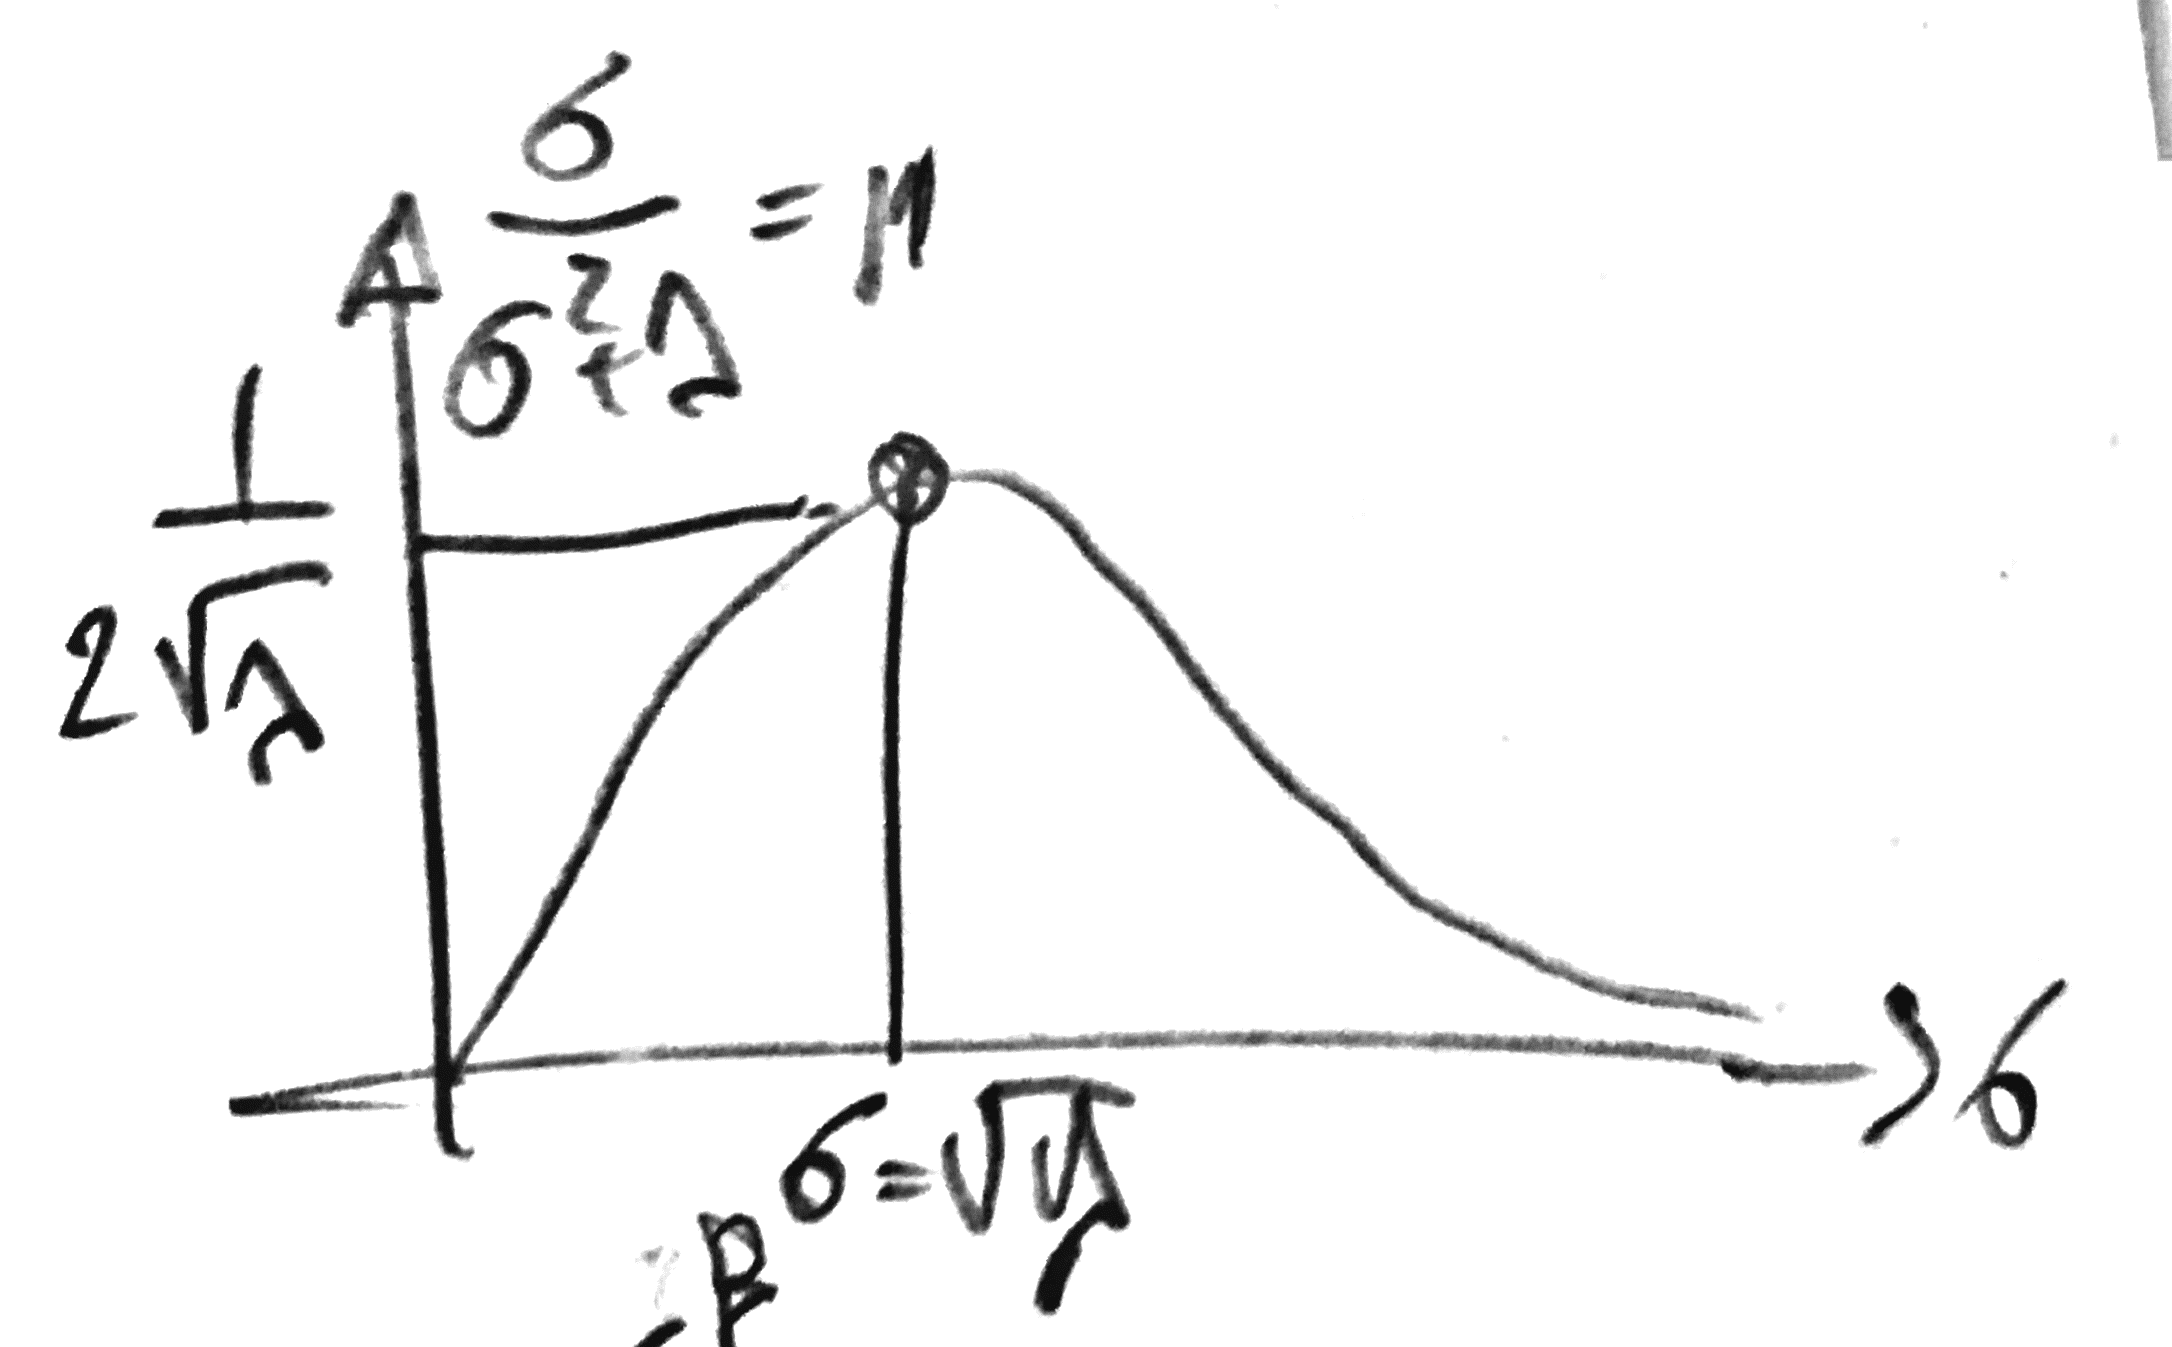
\includegraphics[width=.35\linewidth]{inverse-problems/bound-regul-1} \quad
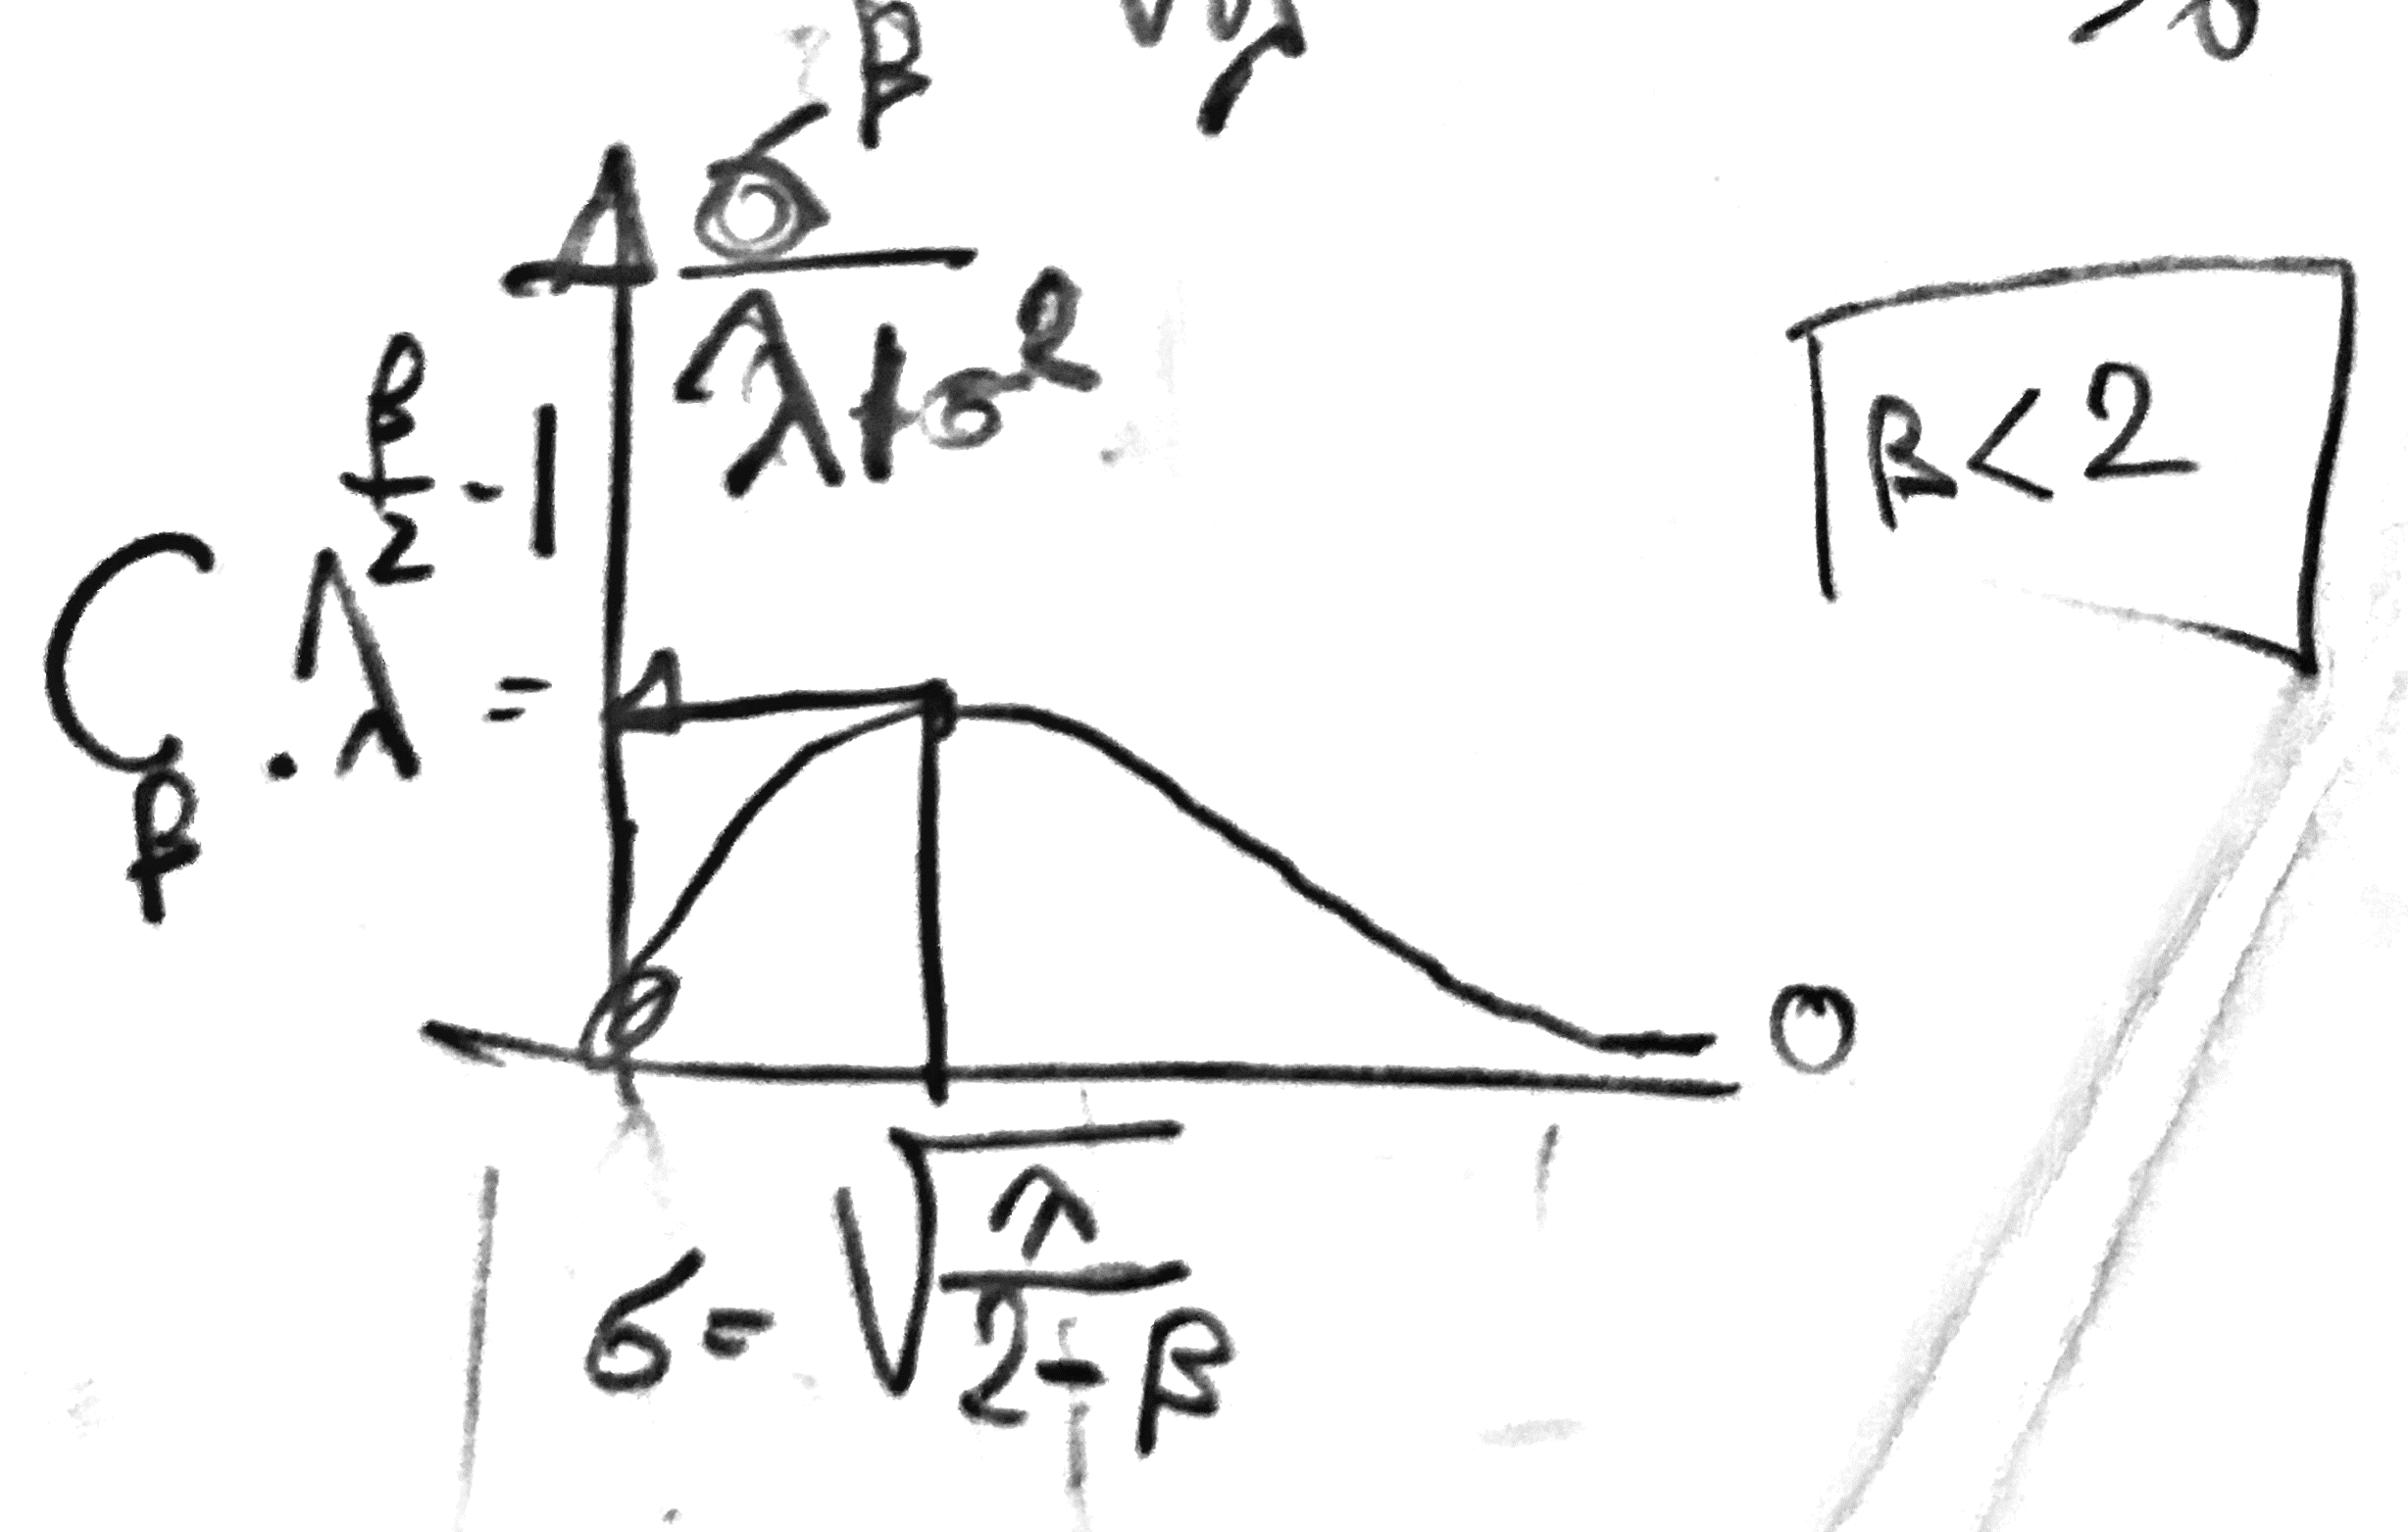
\includegraphics[width=.35\linewidth]{inverse-problems/bound-regul-2}
\caption{\label{fig-bound-regul}
Bounding $\mu_{\la}(\si) \leq C_\la = \frac{1}{2\sqrt{\la}}$ (left)  and 
$\frac{\si^\be}{\la+\si^2} \leq D_{\la,\be}/\la$ (right). 
}
\end{figure}



This theorem shows that using larger $\be \leq 2$ leads to faster convergence rates as $\norm{w}$ drops to zero.
The rate~\eqref{eq-rate-tikhon} however suffers from a ``saturation'' effect, indeed, choosing $\be > 2$ does not helps (it gives the same rate as $\be=2$), and the best possible rate is thus 
\eq{
	\norm{f_\la - f_0} = O( \rho^{\frac{1}{3}} \de^{\frac{2}{3}} ).
}
By choosing more alternative regularization functional $\mu_\la$ and choosing $\be$ large enough, one can show that it is possible to reach rate $\norm{f_\la - f_0} = O( \de^{1-\kappa} )$ for an arbitrary small $\kappa>0$, but one cannot reach a linear rate $\norm{f_\la - f_0}=O(\norm{w})$. Such rates are achievable using non-linear sparse $\ell^1$ regularizations as detailed in Chapter~\ref{chap-sparse-regul}. 

%%%%%%%%%%%%%%%%%%%%%%%%%%%%%%%%%%%%%%%%%%%%%%%%%%%%%%%%%%%%%%%%
%%%%%%%%%%%%%%%%%%%%%%%%%%%%%%%%%%%%%%%%%%%%%%%%%%%%%%%%%%%%%%%%
%%%%%%%%%%%%%%%%%%%%%%%%%%%%%%%%%%%%%%%%%%%%%%%%%%%%%%%%%%%%%%%%
\section{Quadratic Regularization}

After this theoretical study in infinite dimension, we now turn our attention to more practical matters, and focus only on the finite dimensional setting.

%%%%
\paragraph{Convex regularization.}

Following~\eqref{eq-regul-inv}, the ill-posed problem of recovering an approximation of the high resolution image $f_0 \in \RR^N$ from noisy measures $y = \Phi f_0 + w \in \RR^P$ is regularized by solving a convex optimization problem
\eql{\label{eq-ip-regul}
	f_\la \in  \uargmin{ f \in \RR^N }\; \Ee(f) \eqdef \frac{1}{2} \norm{y-\Phi f}^2 + \la J(f)
}
where $\norm{y-\Phi f}^2$ is the data fitting term (here $\norm{\cdot}$ is the $\ell^2$ norm on $\RR^P$) and $J(f)$ is a convex functional on $\RR^N$.

The Lagrange multiplier $\la$ weights the importance of these two terms, and is in practice difficult to set.
Simulation can be performed on high resolution signal $f_0$ to calibrate the multiplier by minimizing the super-resolution error $\norm{f_0-\tilde f}$, but this is usually difficult to do on real life problems.


In the case where there is no noise, $w = 0$, the Lagrange multiplier $\la$ should be set as small as possible. In the limit where $\la \rightarrow 0$, the unconstrained optimization problem~\eqref{eq-ip-regul} becomes a constrained optimization, as the following proposition explains.
%
Let us stress that, without loss of generality, we can assume that $y \in \Im(\Phi)$, because one has the orthogonal decomposition
\eq{
	\norm{y-\Phi f}^2 = \norm{y-\Proj_{\Im(\Phi)}(y)}^2 + \norm{\Proj_{\Im(\Phi)}(y)-\Phi f}^2
}
so that one can replace $y$ by $\Proj_{\Im(\Phi)}(y)$ in~\eqref{eq-ip-regul}. 

Let us recall that a function is coercive if its non-empty levelsets $\enscond{f}{J(f) \leq c}$ are bounded (and hence compact) for all $c$.

\begin{prop}
We assume that $J$ is coercive and that $y \in \Phi$. Then, if for each $\la$, $f_\la$ is a solution of~\eqref{eq-ip-regul}, then $(f_\la)_\la$ is a bounded set and any accumulation point $f^\star$ is a solution of
\eql{\label{eq-ip-regul-noiseless}
	f^\star = \uargmin{f \in \RR^N} \enscond{ J(f) }{ \Phi f = y�}.
}
\end{prop}

\begin{proof}
	Denoting $h$, any solution to~\eqref{eq-ip-regul-noiseless}, which in particular satisfies $\Phi h = y$, because of the optimality condition of $f_\la$ for~\eqref{eq-ip-regul}, one has
	\eq{
		\frac{1}{2\la} \norm{\Phi f_\la-y}^2 + J(f_\la) \leq \frac{1}{2\la} \norm{\Phi h-y}^2 + J(h) = J(h). 
	}
	This shows that $J(f_\la) \leq J(h)$ so that since $J$ is coercive the set $(f_\la)_\la$ is bounded and thus one can consider an accumulation point $f_{\la_k} \rightarrow f^\star$ for $k \rightarrow +\infty$.  Since $\norm{\Phi f_{\la_k}-y}^2 \leq \la_k J(h)$, one has in the limit $\Phi f^\star = y$, so that $f^\star$ satisfies the constraints in~\eqref{eq-ip-regul-noiseless}. Furthermore, by continuity of $J$, passing to the limit in $J(f_{\la_k}) \leq J(h)$, one obtains $J(f^\star) \leq J(h)$ so that $f^\star$ is a solution of~\eqref{eq-ip-regul-noiseless}. 
\end{proof}

Note that it is possible to extend this proposition in the case where $J$ is not necessarily coercive on the full space (for instance the TV functionals in Section~\ref{sec-tv-regul}�bellow) but on the orthogonal to $\ker(\Phi)$. The proof is more difficult.


%%%%
\paragraph{Quadratic Regularization.}

The simplest class of prior functional are quadratic, and can be written as
\eql{\label{eq-quad-regul}
	J(f) = \frac{1}{2}\norm{G f}_{\RR^K}^2 = \frac{1}{2} \dotp{L f}{f}_{\RR^N}
}
where $G \in \RR^{K \times N}$ and 
where $L=G^*G \in \RR^{N \times N}$ is a positive semi-definite matrix.
%
The special case~\eqref{eq-regul-normsq} is recovered when setting $G=L=\Id_N$. 

Writing down the first order optimality conditions for~\eqref{eq-ip-regul} leads to
\eq{
	\nabla \Ee(f) = \Phi^*( \Phi f - y ) + \la L f = 0, 
}
hence, if
\eq{
	\ker(\Phi) \cap \ker(G) = \{0\}, 
}
then~\eqref{eq-quad-regul} has a unique minimizer $f_\la$, which is obtained by solving a linear system
\eql{\label{eq-ip-quad-explicit}
	f_\la = ( \Phi^* \Phi + \la L )^{-1} \Phi^* y.  
}
In the special case where $L$ is diagonalized by the singular basis $(v_m)_m$ of $\Phi$, i.e. $L=V \diag(\al_m^2) V^*$, then $f_\la$ reads in this basis 
\eql{\label{eq-sing-diag-ip}
	\dotp{f_{\la}}{v_m} = \frac{\si_m}{\si_m^2 + \la \al_m^2} \dotp{y}{v_m}.
}


%%%
\paragraph{Example of convolution.}

A specific example is for convolution operator 
\eql{\label{eq-convol-example}
	\Phi f = h \star f, 
}
and using $G=\nabla$ be a discretization of the gradient operator, such as for instance using first order finite differences~\eqref{eq-disc-diff-1}. This corresponds to the discrete Sobolev prior introduced in Section~\ref{subsec-disc-priors}.
%
Such an operator compute, for a $d$-dimensional signal $f \in \RR^N$ (for instance a 1-D signal for $d=1$ or an image when $d=2$), an approximation $\nabla f_n \in \RR^d$ of the gradient vector at each sample location $n$. Thus typically, $\nabla : f \mapsto (\nabla f_n)_n \in \RR^{N \times d}$ maps to $d$-dimensional vector fields.
%
Then $-\nabla^* : \RR^{N \times d} \rightarrow \RR^N$ is a discretized divergence operator.
%
In this case, $\De=-GG^*$ is a discretization of the Laplacian, which is itself a convolution operator. One then has
\eql{\label{eq-quad-regul-convol}
	\hat f_{\la,m} = \frac{\hat h_m^* \hat y_m}{|\hat h_m|^2 - \la \hat d_{2,m}}, 
}
where $\hat d_2$ is the Fourier transform of the filter $d_2$ corresponding to the Laplacian. For instance, in dimension 1, using first order finite differences, the expression for $\hat d_{2,m}$ is given in~\eqref{eq-fft-lapl}.




%%%%%%%%%%%%%%%%%%%%%%%%%%%%%%%%%%%%%%%%%%%%%%%%%%%%%%%%%%%%%%%%
\subsection{Solving Linear System}

When $\Phi$ and $L$ do not share the same singular spaces, using~\eqref{eq-sing-diag-ip} is not possible, so that one needs to solve the linear system~\eqref{eq-ip-quad-explicit}, which can be rewritten as
\eq{
	A f = b \qwhereq A \eqdef \Phi^* \Phi + \la L \qandq b = \Phi^* y. 
} 
It is possible to solve exactly this linear system with direct methods for moderate $N$ (up to a few thousands), and the numerical complexity for a generic $A$ is $O(N^3)$. Since the involved matrix $A$ is symmetric, the best option is to use Choleski factorization $A=BB^*$ where $B$ is lower-triangular. In favorable cases, this factorization (possibly with some re-re-ordering of the row and columns) can take advantage of some sparsity in $A$.

For large $N$, such exact resolution is not an option, and should use approximate iterative solvers, which only access $A$ through matrix-vector multiplication. This is especially advantageous for imaging applications, where such multiplications are in general much faster than a naive $O(N^2)$ explicit computation. If the matrix $A$ is highly sparse, this typically necessitates $O(N)$ operations. 
%
In the case where $A$ is symmetric and positive definite (which is the case here), the most well known method is the conjugate gradient methods, which is actually an optimization method solving
\eql{\label{eq-quad-func}
	\umin{f \in \RR^N} \Ee(f) \eqdef \Qq(f) \eqdef \dotp{A f}{f} - \dotp{f}{b}	
}
which is equivalent to the initial minimization~\eqref{eq-ip-regul}. Instead of doing a naive gradient descent (as studied in Section~\ref{sec-grad-descent} bellow), stating from an arbitrary $\itz{f}$, it compute a new iterate $\iit{f}$ from the previous iterates as
\eq{
	\iit{f} \eqdef \uargmin{f} \enscond{ \Ee(f) }{ f \in \it{f} + \Span(\nabla \Ee(\itz{f}), \ldots,\nabla \Ee(f^{\ell}) ) }.
}
The crucial and remarkable fact is that this minimization can be computed in closed form at the cost of two matrix-vector product per iteration, for $k \geq 1$ (posing initially $\itz{d} = \nabla \Ee(\itz{f}) = A\itz{f}-b$)
\eql{\label{eq-iter-cgs}
	\iit{f} = \it{f} - \tau_\ell \it{d}
	\qwhereq	
	\it{d} =  g_\ell + \frac{ \norm{ \it{g} }^2 }{ \norm{g^{(\ell-1)}}^2 } d^{(\ell-1)}
	\qandq
	\tau_\ell = \frac{
			\dotp{ g_\ell }{\it{d}}
		}{ 
			\dotp{A \it{d}}{\it{d}} 
		}			
}
$\it{g} \eqdef \nabla \Ee(\it{f}) = A\it{f}-b$.
%
It can also be shown that the direction $\it{d}$ are orthogonal, so that after $\ell=N$ iterations, the conjugate gradient computes the unique solution $f^{(\ell)}$ of the linear system $A f = b$.  It is however rarely used this way (as an exact solver), and in practice much less than $N$ iterates are computed.
%
It should also be noted that iterations~\eqref{eq-iter-cgs} can be carried over for an arbitrary smooth convex function $\Ee$, and it typically improves over the gradient descent (although in practice quasi-Newton method are often preferred). 



%%%%%%%%%%%%%%%%%%%%%%%%%%%%%%%%%%%%%%%%%%%%%%%%%%%%%%%%%%%%%%%%
%%%%%%%%%%%%%%%%%%%%%%%%%%%%%%%%%%%%%%%%%%%%%%%%%%%%%%%%%%%%%%%%
%%%%%%%%%%%%%%%%%%%%%%%%%%%%%%%%%%%%%%%%%%%%%%%%%%%%%%%%%%%%%%%%
\section{Non-Quadratic Regularization}

%%%%%%%%%%%%%%%%%%%%%%%%%%%%%%%%%%%%%%%%%%%%%%%%%%%%%%%%%%%%%%%%
\subsection{Total Variation Regularization}
\label{sec-tv-regul}

A major issue with quadratic regularization such as~\eqref{eq-quad-regul} is that they typically leads to blurry recovered data $f_\la$, which is thus not a good approximation of $f_0$ when it contains sharp transition such as edges in images. 
%
This is can clearly be seen in the convolutive case~\eqref{eq-quad-regul-convol}, this the restoration operator $\Phi_\la^+ \Phi$ is a filtering, which tends to smooth sharp part of the data.

This phenomena can also be understood because the restored data $f_\la$ always belongs to $\Im(\Phi^*)=\ker(\Phi)^\bot$, and thus cannot contains ``high frequency'' details that are lost in the kernel of $\Phi$. To alleviate this shortcoming, and recover missing information in the kernel, it is thus necessarily to consider non-quadratic and in fact non-smooth regularization. 

%%
\paragraph{Total variation.}

The most well know instance of such a non-quadratic and non-smooth regularization is the total variation prior. For smooth function $f : \RR^d \mapsto \RR$, this amounts to replacing the quadratic Sobolev energy (often called Dirichlet energy) 
\eq{
	\Jsob(f) \eqdef \frac{1}{2}�\int_{\RR^d} \norm{\nabla f}_{\RR^d}^2 \d x, 
}
where $\nabla f(x) = (\partial_{x_1} f(x), \ldots, \partial_{x_d} f(x))^\top$ is the gradient, by the (vectorial) $L^1$ norm of the gradient
\eq{
	\Jtv(f) \eqdef \int_{\RR^d} \norm{\nabla f}_{\RR^d} \d x.
}
We refer also to Section~\ref{sec-sob-tv-cont} about these priors.
%
Simply ``removing'' the square $^2$ inside the integral might seems light a small change, but in fact it is a game changer. 

Indeed, while $\Jsob(1_{\Om}) = +\infty$ where $1_{\Om}$ is the indicator a set $\Om$ with finite perimeter $|\Om|<+\infty$, one can show that $\Jtv(1_{\Om})=|\Om|$, if one interpret $\nabla f$ as a distribution $Df$ (actually a vectorial Radon measure) and $\int_{\RR^d} \norm{\nabla f}_{\RR^d} \d x$ is replaced by the total mass $|Df|(\Om)$ of this distribution $m=Df$
\eq{
	|m|(\Om) = \sup \enscond{ \int_{\RR^d}�\dotp{h(x)}{\d m(x)} }{h \in \Cc(\RR^d \mapsto \RR^d),  \foralls x, \norm{h(x)} \leq 1 }.
}
The total variation of a function such that $Df$ has a bounded total mass (a so-called bounded variation function) is hence defined as
\eq{
	\Jtv(f) \eqdef \sup \enscond{  \int_{\RR^d} f(x) \diverg(h)(x) \d x  }{ h \in \Cc^1_c(\RR^d;\RR^d), \norm{h}_\infty \leq 1 }.
}
Generalizing the fact that $\Jtv(1_\Om)=|\Om|$, the functional co-area formula reads
\eq{
	\Jtv(f) = \int_\RR \Hh_{d-1}( L_t(f) ) \d t
	\qwhereq
	L_t(f) = \enscond{x}{f(x)=t}
}
and where $\Hh_{d-1}$ is the Hausforf measures of dimension $d-1$, for instance, for $d=2$ if $L$ has finite perimeter $|L|$, then $\Hh_{d-1}(L)=|L|$ is the perimeter of $L$.


%%
\paragraph{Discretized Total variation.}

For discretized data $f \in \RR^N$, one can define a discretized TV semi-norm as detailed in Section~\ref{subsec-disc-priors}, and it reads, generalizing~\eqref{eq-discr-tv} to any dimension
\eq{
	\Jtv(f) = \sum_n \norm{\nabla f_n}_{\RR^d}
}
where $\nabla f_n \in \RR^d$ is a finite difference gradient at location indexed by $n$. 


The discrete total variation prior $\Jtv(f)$ defined in \eqref{eq-discr-tv} is a convex but non differentiable function of $f$, since a term of the form $\norm{\nabla f_n}$ is non differentiable if $\nabla f_n=0$.
%
We defer to chapters~\ref{chap-convex-optim}�and~\ref{chap-conv-duality}�the study of advanced non-smooth convex optimization technics that allows to handle this kind of functionals.

In order to be able to use simple gradient descent methods, one needs to smooth the TV functional. The general machinery proceeds by replacing the non-smooth $\ell^2$ Euclidean norm $\norm{\cdot}$ by a smoothed version, for instance
\eq{
	\foralls u \in \RR^d, \quad \norm{u}_\epsilon \eqdef \sqrt{ \epsilon^2 + \norm{u} }.
}
This leads to the definition of a smoothed approximate TV functional, already introduced in~\eqref{eq-tv-smoothed}, 
\eq{
	\Jtv^\epsilon(f) \eqdef \sum_n \norm{\nabla f_n}_\epsilon
}
One has the following asymptotics for $\epsilon \rightarrow \{0,+\infty\}$
\eq{
	\norm{u}_\epsilon \overset{\epsilon\rightarrow 0}{\longrightarrow}	\norm{u}
	\qandq
	\norm{u}_\epsilon = \epsilon + \frac{1}{2\epsilon} \norm{u}^2 + O(1/\epsilon^2)
}
which suggest that $\Jtv^\epsilon$ interpolates between $\Jtv$ and $\Jsob$.

The resulting inverse  regularization problem~\eqref{eq-ip-regul} thus reads 
\eql{\label{eq-ip-tv-eps}
	f_\la \eqdef \uargmin{f \in \RR^N} \Ee(f) = \frac{1}{2}\norm{y-\Phi f}^2 + \la \Jtv^\epsilon(f)
}
It is a strictly convex problem (because $\norm{\cdot}_\epsilon$ is strictly convex for $\epsilon>0$) so that its solution $f_\la$ is unique. 



%%%%%%%%%%%%%%%%%%%%%%%%%%%%%%%%%%%%%%%%%%%%%%%%%%%%%%%%%%%%%%%%
\subsection{Gradient Descent Method}
\label{sec-grad-descent}

The optimization program~\eqref{eq-ip-tv-eps} is a example of smooth unconstrained convex optimization of the form
\eql{\label{eq-min-smooth-uncons-ip}
	\umin{f \in \RR^N} \Ee(f)
}
where $\Ee : \RR^N \rightarrow \RR$ is a $\Cc^1$ function. Recall that the gradient $\nabla \Ee : \RR^N \mapsto \RR^N$ of this functional (not to be confound with the discretized gradient $\nabla f \in \RR^N$ of $f$) is defined by the following first order relation
\eq{
	\Ee(f+r) = \Ee(f) + \dotp{f}{r}_{\RR^N} + O(\norm{r}_{\RR^N}^2)
}
where we used $O(\norm{r}_{\RR^N}^2)$ in place of $o(\norm{r}_{\RR^N})$ (for differentiable function) because we assume here $\Ee$ is of class $\Cc^1$ (i.e. the gradient is continuous). 

For such a function, the gradient descent algorithm is defined as
\eql{\label{eq-grad-desc}
	\iit{f} \eqdef \it{f} - \tau_\ell \nabla \Ee( \it{f} ), 
}
where the step size $\tau_\ell>0$ should be small enough to guarantee convergence, but large enough for this algorithm to be fast.

We refer to Section~\ref{sec-grad-descent} for a detailed analysis of the convergence of the gradient descent, and a study of the influence of the step size $\tau_\ell$.



%%%%%%%%%%%%%%%%%%%%%%%%%
\subsection{Examples of Gradient Computation}
\label{eq-example-grad}

Note that the gradient of a quadratic function $\Qq(f)$ of the form~\eqref{eq-quad-func} reads
\eq{
	\nabla \Gg(f) = Af-b.
}
In particular, one retrieves that the first order optimality condition $\nabla \Gg(f)=0$ is equivalent to the linear system $Af=b$. 

For the quadratic fidelity term $\Gg(f)=\frac{1}{2}\norm{\Phi f-y}^2$, one thus obtains
\eq{
	\nabla \Gg(f) = \Phi^*(\Phi y - y). 
}

In the special case of the regularized TV problem~\eqref{eq-ip-tv-eps}, the gradient of $\Ee$ reads
\eq{
	\nabla \Ee(f) = \Phi^*(\Phi y - y) + \la \nabla \Jtv^\epsilon(f).
}
Recall the chain rule for differential reads $\partial (\Gg_1 \circ \Gg_2) = \partial \Gg_1 \circ \partial \Gg_2$, but that gradient vectors are actually transposed of differentials, so that for $\Ee = \Ff \circ \Hh$ where $\Ff : \RR^P \rightarrow \RR$ and $\Hh : \RR^N \rightarrow \RR^P$, one has
\eq{
	\nabla \Ee(f) = [ \partial \Hh( f ) ]^*\pa{ \nabla \Ff( \Hh f ) }.�
}

Since $\Jtv^\epsilon = \norm{\cdot}_{1,\epsilon} \circ \nabla$, one thus has
\eq{
	\nabla \Jtv^\epsilon = \nabla^\star \circ ( \partial \norm{\cdot}_{1,\epsilon} )
	\qwhereq
	\norm{u}_{1,\epsilon} = \sum_n \norm{u_n}_\epsilon
}
so that 
\eq{
	\Jtv^\epsilon(f) = -\diverg( \Nn^\epsilon( \nabla f) ), 
}
where $\Nn^\epsilon(u) = ( u_n/\norm{u_n}_\epsilon )_n$ is the smoothed-normalization operator of vector fields (the differential of $\norm{\cdot}_{1,\epsilon}$), and where $\diverg=-\nabla^*$ is minus the adjoint of the gradient.

Since $\diverg=-\nabla^*$, their Lipschitz constants are equal $\norm{\diverg}_\text{op}=\norm{\nabla}_\text{op}$, and is for instance equal to $\sqrt{2d}$ for the discretized gradient operator. 
%
Computation shows that the Hessian of $\norm{\cdot}_\epsilon$ is bounded by $1/\epsilon$, so that for the smoothed-TV functional, the Lipschitz constant of the gradient is upper-bounded by
\eq{
	L = \frac{\norm{\nabla}^2}{\epsilon} + \norm{\Phi}_{\text{op}}^2.
}
Furthermore, this functional is strongly convex because $\norm{\cdot}_\epsilon$ is $\epsilon$-strongly convex, and the Hessian is lower bounded by
\eq{
	\mu = \epsilon + \si_{\min}( \Phi )^2
}
where $\si_{\min}( \Phi )$ is the smallest singular value of $\Phi$. For ill-posed problems, typically $\si_{\min}( \Phi )=0$ or is very small, so that both $L$ and $\mu$ degrades (tends respectively to $0$ and $+\infty$) as $\epsilon \rightarrow 0$, so that gradient descent becomes prohibitive for small $\epsilon$, and it is thus required to use dedicated non-smooth optimization methods detailed in the following chapters. 
%
On the good news side, note however that in many case, using a small but non-zero value for $\epsilon$ often leads to better a visually more pleasing results, since it introduce a small blurring which diminishes the artifacts (and in particular the so-called ``stair-casing'' effect) of TV regularization. 



%%%%%%%%%%%%%%%%%%%%%%%%%%%%%%%%%%%%%%%%%%%%%%%%%%%%%%%%%%%%%%%%
%%%%%%%%%%%%%%%%%%%%%%%%%%%%%%%%%%%%%%%%%%%%%%%%%%%%%%%%%%%%%%%%
%%%%%%%%%%%%%%%%%%%%%%%%%%%%%%%%%%%%%%%%%%%%%%%%%%%%%%%%%%%%%%%%
\section{Examples of Inverse Problems}

We detail here some inverse problem in imaging that can be solved using quadratic regularization or non-linear TV.

%%%%%%%%%%%%%%%%%%%%%%%%%%%%%%%%%%%%%%%%%%%%%%%%%%%%%%%%%%%%%%%%
\subsection{Deconvolution}
\label{subsec-deconv}

The blurring operator \eqref{eq-deblurring-operator} is diagonal over Fourier, so that quadratic regularization are easily solved using Fast Fourier Transforms when considering periodic boundary conditions. We refer to~\eqref{eq-convol-example} and the correspond explanations. TV regularization in contrast cannot be solved with fast Fourier technics, and is thus much slower.


%%%%%%%%%%%%%%%%%%%%%%%%%%%%%%%%%%%%%%%%%%%%%%%%%%%%%%%%%%%%%%%%
\subsection{Inpainting}
\label{sec-inpainting-variational}

For the inpainting problem, the operator defined in \eqref{eq-inp-operator} is diagonal in space
\eq{
	 \Phi = \diag_m( \de_{\Om^c}[m] ),
}
and is an orthogonal projector $\Phi^* = \Phi$.

In the noiseless case, to constrain the solution to lie in the affine space $\enscond{f \in \RR^N}{y=\Phi f}$, we use the orthogonal projector
\eq{
	\foralls x, \quad P_y(f)(x) = \choice{
		f(x) \qifq x \in \Om,\\
		\; y(x) \quad \qifq x \notin \Om.
	}
}


In the noiseless case, the recovery \eqref{eq-ip-regul-noiseless} is solved using a projected gradient descent.
For the Sobolev energy, the algorithm iterates
\eq{
	\iit{f}= P_y( \it{f} + \tau \Delta \it{f} ).
}
which converges if $\tau < 2 / \norm{\Delta} = 1/4$. Figure \ref{fig-inp-sob-iter} shows some iteration of this algorithm, which progressively interpolate within the missing area. 

% Table \ref{inverse-inpainting-sob} details the implementation of the inpainting with the Sobolev prior.

%\matlab{matlab/inverse-inpainting-sob.m
%}{
%Inpainting with Sobolev regularization. The mask $\Om$ is given in \matvar{mask}, so that the masked indices are \matvar{f(mask)}, the observations in \matvar{y}. The solution is given in \matvar{fsob}.
%}{inverse-inpainting-sob}

\myfigure{
\tabquatre{
\image{invpbm}{.24}{sob-inp-iter-1}&
\image{invpbm}{.24}{sob-inp-iter-2}&
\image{invpbm}{.24}{sob-inp-iter-3}&
\image{invpbm}{.24}{sob-inp-iter-4} \\
$k=1$ & $k=10$ & $k=20$ & $k=100$ 
}
}{%
	Sobolev projected gradient descent algorithm. %	
}{fig-inp-sob-iter}

%\myfigure{
%\tabdeux{
%\image{invpbm}{.3}{sob-inp-decay-conv}&
%\image{invpbm}{.3}{sob-inp-decay-energy} \\
%$\log_{10}( E(\it{f})/E(f^\star)-1 )$ &
%$\log_{10}( \norm{\it{f}-f^\star}/\norm{f_0} )$
%}
%}{%
%	Decay of the energy and convergence for Sobolev inpainting.%	
%}{fig-sob-inp-decay}

Figure \ref{fig-inpainting-parrot} shows an example of Sobolev inpainting to achieve a special effect.

\myfigure{
\tabtrois{
\image{invpbm}{.3}{inpainting-parrot-image}&
\image{invpbm}{.3}{inpainting-parrot-mask}&
\image{invpbm}{.3}{inpainting-parrot-sobolev}\\
Image $f_0$ & Observation $y=\Phi f_0$ & Sobolev $f^\star$ \\
}
}{%
	Inpainting the parrot cage. %	
}{fig-inpainting-parrot}

For the smoothed TV prior, the gradient descent reads
\eq{
	\iit{f}= P_y\pa{
			\it{f} + \tau \diverg\pa{ \frac{ \nabla \it{f}}{ \sqrt{\epsilon^2+\norm{\nabla \it{f}}^2} } }
		}
}
which converges if $\tau < \epsilon/4$.

Figure \ref{fig-inpainting-cameraman} compare the Sobolev inpainting and the TV inpainting for a small value of $\epsilon$. The SNR is not improved by the total variation, but the result looks visually slightly better.

% For special effects : $\Ldeux$ error and SNR are not good measures of quality, $f^\star$ is very different from $f_0$ ! Pereceptual metric, visual inspection.

\myfigure{
\tabdeux{
\image{invpbm}{.3}{inpainting-cameraman-image}&
\image{invpbm}{.3}{inpainting-cameraman-observations}\\
Image $f_0$ & Observation $y=\Phi f_0$ \\
\image{invpbm}{.3}{inpainting-cameraman-sobolev}&
\image{invpbm}{.3}{inpainting-cameraman-tv} \\
Sobolev $f^\star$ & TV $f^\star$ \\
SNR=?dB & SNR=?dB 
}
}{%
	Inpainting with Sobolev and TV regularization. %	
}{fig-inpainting-cameraman}



%%%%%%%%%%%%%%%%%%%%%%%%%%%%%%%%%%%%%%%%%%%%%%%%%%%%%%%%%%%%%%%%
\subsection{Tomography Inversion}

In medical imaging, a scanner device compute projection of the human body along rays $\De_{t,\th}$ defined
\eq{
	x \cdot \tau_\theta = x_1 \cos\th + x_2\sin\th = t
}
where we restrict ourself to 2D projection to simplify the exposition.

The scanning process computes a Radon transform, which compute the integral of the function to acquires along rays
\eq{
	\foralls \th \in [0,\pi), \foralls t \in \RR, \quad
	p_{\th}(t) = \int_{\De_{t,\th}} f(x) \,d s
	 = \iint f(x)\, \de( x \cdot \tau_\theta - t )\, d x 
}
see Figure \eqref{fig-tomo-principle}

\myfigure{
\image{invpbm}{.4}{tomo-principle}
}{%
	Principle of tomography acquisition. %	
}{fig-tomo-principle}

The Fourier slice theorem relates the Fourier transform of the scanned data to the 1D Fourier transform of the data along rays
\eql{\label{eq-fourier-slice}
	\foralls \th \in [0,\pi)~,~ 
\foralls \xi \in \RR\quad
		\hat p_\th(\xi) = \hat f( \xi \cos \th, \xi \sin \th ).
}
This shows that the pseudo inverse of the Radon transform is computed easily over the Fourier domain using inverse 2D Fourier transform
\eq{
	f(x) = 
\frac{1}{2\pi} \int_{0}^\pi p_\th \star h(x \cdot \tau_\theta)\, d \th
}
with $\hat h(\xi) = |\xi|$.


\myfigure{
\tabtrois{
% \image{invpbm}{.4}{tomo-radon}
\image{invpbm}{.3}{tomo-image}&
\image{invpbm}{.35}{tomo-radon-subsample}&
\image{invpbm}{.3}{tomo-radon-fourier}\\
Image $f$ & Radon sub-sampling & Fourier domain
}
}{%
	Partial Fourier measures. %	
}{fig-tomo-radon-subsample}


Imaging devices only capture a limited number of equispaced rays at orientations $\{ \th_k = \pi/k \}_{0 \leq k < K}$. This defines a tomography operator which corresponds to a partial Radon transform
\eq{
	R f = ( p_{\th_k} )_{0 \leq k < K}.
}
Relation \eqref{eq-fourier-slice} shows that knowing $R f$ is equivalent to knowing the Fourier transform of $f$ along rays, 
\eq{
	\{ \hat f(\xi \cos(\th_k), \xi \sin(\th_k))�\}_k.
}
We thus simply the acquisition process over the discrete domain and model it as computing directly samples of the Fourier transform 
\eq{
	\Phi f = ( \hat f[\om] )_{\om \in \Om} \in \RR^P
}
where $\Om$ is a discrete set of radial lines in the Fourier plane, see Figure \ref{fig-tomo-radon-subsample}, right.

In this discrete setting, recovering from Tomography measures $y=R f_0$ is equivalent in this setup to inpaint missing Fourier frequencies, and we consider partial noisy Fourier measures
\eq{
	\foralls \om \in \Om, \quad y[\om] = \hat f[\om] + w[\om]
}
where $w[\om]$ is some measurement noise, assumed here to be Gaussian white noise for simplicity.

\myfigure{
\tabtrois{
\image{invpbm}{.3}{tomo-image}&
\image{invpbm}{.3}{tomo-pinv-13}&
\image{invpbm}{.3}{tomo-pinv-32}\\
Image $f_0$ & 13 projections & 32 projections.
}
}{%
	Pseudo inverse reconstruction from partial Radon projections. %	
}{fig-tomo-pinv}

The peuso-inverse $f^+ = R^+ y$ defined in \eqref{eq-pseudo-inverse} of this partial Fourier measurements  reads 
\eq{
	{\hat f}^+[\om] = \choice{
		y[\om] \qifq \om \in \Om,\\
		\; 0 \qifq \om \notin \Om.
	}
}
Figure \ref{fig-tomo-pinv} shows examples of pseudo inverse reconstruction for increasing size of $\Om$. This reconstruction exhibit serious artifact because of bad handling of Fourier frequencies (zero padding of missing frequencies).

The total variation regularization \eqref{eq-tv-dn} reads
\eq{
	f^\star \in \uargmin{f} \frac{1}{2}\sum_{\om \in \Om} |y[\om] - \hat f[\om]|^2 
	+ \la \normTV{f}.
}
It is especially suitable for medical imaging where organ of the body are of relatively constant gray value, thus resembling to the cartoon image model introduced in Section \ref{subsec-cartoon-images}. Figure \ref{fig-tomo-tv} compares this total variation recovery to the pseudo-inverse for a synthetic cartoon image. This shows the hability of the total variation to recover sharp features when inpainting Fourier measures. This should be contrasted with the difficulties that faces TV regularization to inpaint over the spacial domain, as shown in Figure \ref{fig-inpainting-lena}.

\myfigure{
\tabtrois{
\image{invpbm}{.3}{tomo-image}&
\image{invpbm}{.3}{tomo-pinv-fourier}&
\image{invpbm}{.3}{tomo-tv}\\
Image $f_0$ & Pseudo-inverse & TV
}
}{%
	Total variation tomography inversion. %	
}{fig-tomo-tv}
